
\chapter[Partial Differential Equations]{Finite difference methods for Partial Differential Equations}

\section[Revision]{Revision of Partial Differential Equations}

A {\em partial differential equation} is a relation between the
partial derivatives of an unknown function and the independent
variables.  The order of the highest derivative is called the {\em
  order} of the equation.

Just as in the case of an ordinary differential equation, we say that
a partial differential equation is {\em linear} if it is of the first
degree in the dependent variable (the unknown function) and its
partial derivatives.  If each term of such equation contains either
the dependent variable or one of its derivatives, the equation is
called {\em homogeneous}; otherwise it is said to be {\em non
  homogeneous}.

\smallskip

\noindent
{\bf Example} - The equations
%
\begin{align*}
  (a) & & \pdv{\phi}{t} - \pdv[2]{\phi}{x} &= 0, \\
  (b) & & \phi(x,t) \pdv[2]{\phi}{t} + \pdv{\phi}{x} &= f(x,t), \\
  (c) & & \pdv[4]{\phi}{x} + \pdv[4]{\phi}{y} &= g(x,y) ,
\end{align*}
%
are, respectively, (a) Linear, homogeneous, second order, (b)
nonlinear, non-homogeneous, second order, (c) linear, non-homogeneous,
fourth order.

\smallskip

In this unit we consider only second order linear partial differential
equations with constant coefficients:
%
\begin{equation*}
  A \pdv[2]{u}{x} + 2 B \pdv{u}{x}{y} +
  C \pdv[2]{u}{y} + D \pdv{u}{x} + E \pdv{u}{y} = f(x,y) .
\end{equation*}
%
These equations are classified in three groups\footnote{Note that the
  coefficients $A$, $B$, etc. need not be constant}:

\medskip

\begin{center}
  \begin{tabular}{|l|l|l|l|} \hline
    \multicolumn{1}{|c|}{ Type} &
    \multicolumn{1}{c|}{Coefficients} &
    \multicolumn{1}{c|} {Typical form} &
    \multicolumn{1}{c|} {Name} \\ \hline \hline
    Hyperbolic & $B^2 - 4 A C > 0 $ &
    $u_{t t} - c^2 u_{x x} = 0 $ & Wave eq. \\ \hline
    Parabolic & $B^2 - 4 A C = 0 $ &
    $u_{t} - c^2 u_{x x} = 0 $ & Heat eq. \\ \hline
    Elliptic & $B^2 - 4 A C < 0 $ &
    $u_{x x} + u_{y y} = 0 $ & Laplace eq. \\ \hline
  \end{tabular}
\end{center}

\medskip

\noindent
The names arise by analogy with the curve
%
\begin{equation*}
  a x^2 + 2 b x y + c y^2 = f,
\end{equation*}
%
which represents an hyperbola, parabola and ellipse according as $b^2
- 4 a c$ is positive, zero or negative, respectively.

The classification of the equations is very important for the study of
their solutions.  A {\em solution} of a partial differential equation
in some region $R$ of the space of the independent variables is a
function that has all the partial derivatives that appear in the
equation and that satisfies the equation everywhere in $R$.  Like
ordinary differential equations, Partial differential equation have
many solutions.  For example, the functions
%
\begin{equation*}
  u(x,y) = x^2 - y^2, \quad u = e^x \cos(y), \quad u=\ln(x^2+y^2),
\end{equation*}
%
are all solutions of the equation
%
\begin{equation*}
  \pdv[2]{u}{x} + \pdv[2]{u}{y} = 0 .
\end{equation*}
%
Exactly like for ordinary differential equations we must specify
something more if we wish to obtain a unique solution: for example we
must specify the value of the function on the boundary of the region
$R$ ({\em boundary conditions}), and/or we must specify the value of
the function at the start ({\em initial conditions}).  What type of
boundary or initial condition to use depends on the type of Partial
differential equation.

\medskip

\centerline{\bf Hyperbolic}

\noindent \underline{Example}: $u_{t t} - c^2 u_{xx} = 0$.

\noindent \underline{Physical meaning}: Wave motion

\noindent \underline{Initial conditions}: The value of $u$ and its
time derivative at $t=0$: $u(x,0)=f(x)$ and $u_t(x,0)=g(x)$.

\noindent \underline{Boundary conditions}: Either $u$ or its normal
derivative at the boundary of the integration region: e.g.\ $u(0,t) =
\phi_1(t)$ and $u(L,t)= \phi_2(t)$.  The former type of boundary
condition is called a \textit{Dirichlet} boundary condition; the
latter is called a \textit{Neumann} boundary condition.  It is also
possible to mix the two types of boundary conditions (\textit{mixed
  boundary conditions}).

\bigskip

\centerline{\bf Parabolic}

\noindent \underline{Example}: $u_{t} - c^2 u_{xx} = 0$.

\noindent \underline{Physical meaning}: Heat diffusion

\noindent \underline{Initial conditions}: The value of $u$ at $t=0$:
$u(x,0)=f(x)$.

\noindent \underline{Boundary conditions}: Either $u$ or its normal
derivative at the boundary of the integration region: e.g.\ $u(0,t) =
\phi_1(t)$ and $u(L,t)= \phi_2(t)$.

\bigskip

\centerline{\bf Elliptic}

\noindent \underline{Example}: $u_{xx} + u_{y y} = 0$ (Laplace's
equation).

\noindent \underline{Physical meaning}: Stationary profile of a
membrane, stationary temperature profile of a metal plate,
electrostatic potential in the absence of charges.

\noindent \underline{Initial conditions}: They do not apply to these
equations.

\noindent \underline{Boundary conditions}: Either $u$ or its normal
derivative at the boundary of the integration region: e.g.\ if the
region is the rectangle $0 \le x \le a$, $0 \le y \le b$: $u(0,y) =
\phi_1(y)$, $u(a,y)= \phi_2(y)$, $u(x,0) = g_1(x)$ and, finally,
$u(x,b)=g_2(x)$.

\begin{figure}
  \centerline{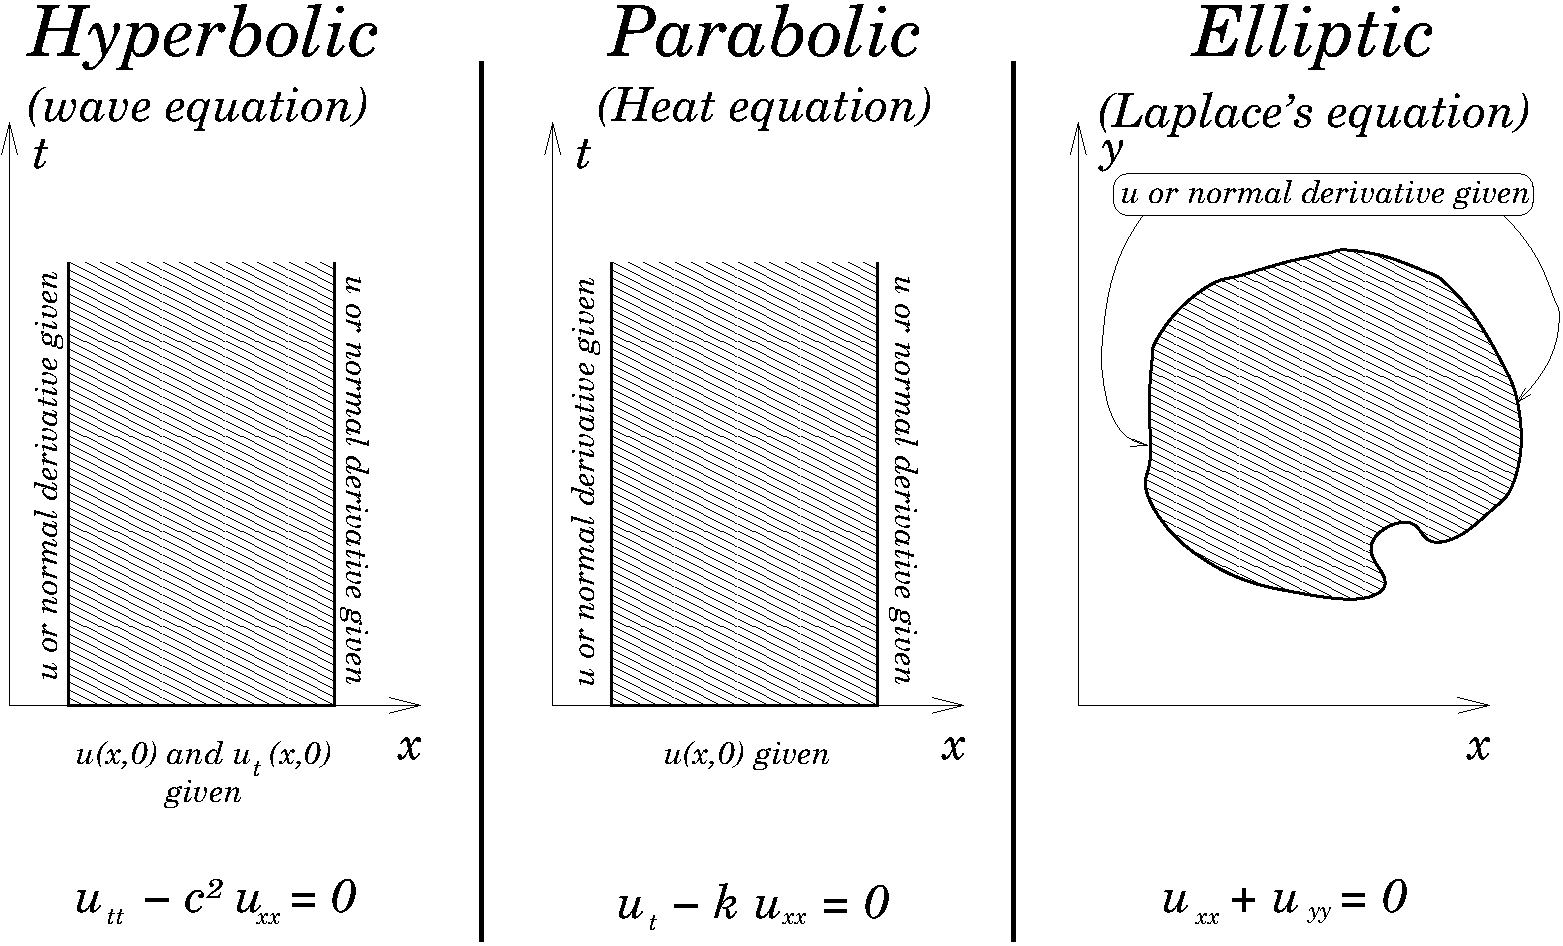
\includegraphics[width=120mm]{figures/pde_summary}}
  \caption{\label{fig:pde_summary} \it Types of partial differential
    equations and their boundary and initial conditions.}
\end{figure}

\section{Numerical methods for PDEs}

There are many classes of methods to solve numerically partial
differential equations.  Three main groups are:

\begin{enumerate}
  %
\item \textit{Finite difference methods}

  The differential operators are approximated using their finite
  difference representation on a given grid.  In this way the Partial
  Differential Equation is transformed to a (nonlinear) algebraic
  equation for the values of the solution on the grid points.  These
  are the only methods that we discuss at any length in this unit.
  %
\item \textit{Finite element methods}

  The domain of the solution is divided into cells.  The solution is
  represented as a simple function (e.g.\ a linear function) on each
  cell and the partial differential equation is transformed to an
  algebraic problem for the matching conditions of the simple
  solutions at the boundaries of the cells.
  %
\item \textit{Spectral methods}

  The solution is represented by a superposition of known functions
  (e.g.\ trigonometric functions or special polynomials).  The partial
  differential equation is transformed to a set of algebraic equations
  or ordinary differential equations for the amplitudes of the
  component functions.  A subclass of these methods are the
  \textit{collocation methods}: the solution is represented on a grid
  and the decomposition of the solution in known functions is used to
  estimate to a high degree of accuracy the partial derivatives of the
  solution on the grid points.  These methods are highly accurate and
  fast, but in general require the domain of the solution to be fairly
  simple, e.g.\ a rectangle.
  %
\end{enumerate}

\section[Elliptic Equations]{Elliptic Equations}

\subsection{Introduction}

A ``standard form'' of elliptic partial differential equation with
Dirichlet boundary conditions is
%
\begin{equation}
  \left\{
    \begin{aligned}
      u_{xx} + u_{y y} & = f(x,y), & & {\rm in}~~\Omega,\\
      u\big |_{\partial\Omega} & = \phi(x,y), & & {\rm on}~~\partial\Omega.
    \end{aligned}
  \right.\label{dp}
\end{equation}
%
This problem has a unique solution if the domain $\Omega$ has a smooth
boundary and $f$ and $\phi$ are continuous functions.

\subsection{A simple finite difference method}

We are going to solve equation~(\ref{dp}) numerically using the method
of finite differences.  At the heart of this method is the finite
difference approximation of the second derivative of a function
$y(x)$:
%
\begin{equation}
  y''(x) = \frac{1}{h^2}[y(x+h)+y(x-h)-2y(x)]-
  \frac{h^2}{12}y^{(4)}(\xi), \label{fd}
\end{equation}
%
where $h$ is a fixed step size.  We illustrate this method using a
simple case of equation~(\ref{dp}), namely the case of a Dirichlet
problem on a rectangle $0<x<a$, $0<y<b$.  First, a network of grid
points is established on the rectangle:
%
\begin{equation*}
  (x_i,y_j)=(i h_x,j h_y), \qquad 0\le i\le n+1, \quad 0\le j\le m+1,
\end{equation*}
%
where the step sizes in the $x$ and $y$ directions are given by
\begin{equation*}
  h_x=\frac{a}{n+1}, \qquad h_y=\frac{b}{m+1}.
\end{equation*}
%
Next, the differential equation in (\ref{dp}) at the mesh point
$(x_i,y_j)$ is replaced by its finite-difference analogue at that
point, which for $1 \le i \le n$ and $1 \le j \le m$ is:
%
\begin{align}
  \label{eq:ellfd}
  & & \frac{1}{h_x^2}[u_{i-1,j}+u_{i+1,j}-2u_{i,j}] +
  \frac{1}{h_y^2}[u_{i,j-1}+u_{i,j+1}-2u_{i,j}] & = f_{i j},
  \nonumber \\
  \implies & & u_{i-1,j}+u_{i+1,j}-2u_{i,j} + \alpha
  [u_{i,j-1}+u_{i,j+1}-2u_{i,j}] & = h^2f_{i,j},
\end{align}
%
where $u_{i,j} = u(x_i,x_j)$, $\alpha=(h_x/h_y)^2$ and $h=h_x$.  The
values of $u_{i,j}$ are known when $i=0$ or $n+1$ and when $j=0$ or
$m+1$, since these are the prescribed boundary values in the problem:
%
\begin{align*}
  u_{0,j} & = \phi(x_0,y_j)  = \phi(0,y_j) , &
  u_{i,0} & = \phi(x_i,y_0)  = \phi(x_i,0), \\
  u_{n+1,j} & = \phi(x_{n+1},y_j)  = \phi(a,y_j), &
  u_{i,m+1} & = \phi(x_i,y_{m+1})  = \phi(x_i,b).
\end{align*}
%
This means that equation~(\ref{dp}) has been transformed to a
non-homogeneous system of linear equations, given by~(\ref{eq:ellfd}),
with unknowns $u_{i,j}$ and $1\le i\le n$, $1\le j\le m$.

As an example, consider the simple case $n=2$ and $m=3$.  The
approximate solution of equation~(\ref{dp}) at the grid points are the
solution of the $6\times 6$ system
%
\begin{align*}
  [u_{01}-2u_{11}+u_{21}]+\alpha[u_{10}-2u_{11}+u_{12}] &= h^2 f_{11},\\
  [u_{02}-2u_{12}+u_{22}]+\alpha[u_{11}-2u_{12}+u_{13}] &= h^2 f_{12},\\
  [u_{03}-2u_{13}+u_{23}]+\alpha[u_{12}-2u_{13}+u_{14}] &= h^2 f_{13},\\
  [u_{11}-2u_{21}+u_{31}]+\alpha[u_{20}-2u_{21}+u_{22}] &= h^2 f_{21},\\
  [u_{12}-2u_{22}+u_{32}]+\alpha[u_{21}-2u_{22}+u_{23}] &= h^2 f_{22},\\
  [u_{13}-2u_{23}+u_{33}]+\alpha[u_{22}-2u_{23}+u_{24}] &= h^2 f_{23}.
\end{align*}
%
The unknown quantities in this problem can be ordered in many ways. We
select the one known as the natural ordering
%
\begin{equation*}
  u=[u_{11},u_{12},u_{13},u_{21},u_{22},u_{23}]^T.
\end{equation*}
%
The system has the form $A \bu = \bF$ with
%
\begin{equation}
  A = \begin{pmatrix}
      -2 (1+\alpha) & \alpha & 0 & 1 & 0 & 0 \\
      \alpha & -2(1+\alpha) & \alpha & 0 & 1 & 0 \\
      0 & \alpha & -2(1+\alpha) & 0 & 0 & 1 \\
      1 & 0 & 0 & -2(1+\alpha) & \alpha & 0 \\
      0 & 1 & 0 & \alpha & -2(1+\alpha) & \alpha \\
      0 & 0 & 1 & 0 & \alpha & -2(1+\alpha) \\
    \end{pmatrix} \label{eq:PDE:A}
\end{equation}
%
and
%
\begin{equation*}
  \bF =
  \begin{pmatrix}
    h^2f_{11}- u_{01}-\alpha u_{10} \\
    h^2f_{12}- u_{02} \\
    h^2f_{13}- u_{03}-\alpha u_{14} \\
    h^2f_{21}- u_{31}-\alpha u_{20} \\
    h^2f_{22}- u_{32} \\
    h^2f_{23}- u_{33}-\alpha u_{24}
  \end{pmatrix},
\end{equation*}
%
where in the expressions of the components of the vector $\bF$ only
the boundary values of $u_{i,j}$ are present.

In general, the $n\times m$ system is sparse because each equation
contains at most five unknowns.  Iterative procedures such as the
Gauss-Seidel iterative method can be quite effective in this
situation.  Moreover, in setting up such a procedure there is no need
to store the matrix $A$ of the coefficients defined in
equation~(\ref{eq:PDE:A}).  In fact, we can rewrite
equation~(\ref{eq:ellfd}) as
%
\begin{align}
  u_{i,j} &= \frac{1}{2(1+\alpha)} \left [ u_{i-1,j} +u_{i+1,j} +
    \alpha (u_{i,j-1}+u_{i,j+1}) - h^2 f_{i,j} \right ],
    \label{PDE:eq:Ell:Updateuij} \\ & \notag \qquad
  1 \le i \le n, \, 1 \le j \le m .
\end{align}
%
This equation is a Gauss-Seidel formula to update $u_{i,j}$. When this
equation is used, the value obtained from the right-hand side replaces
the old value of $u_{i,j}$.  It can also be seen as an implementation
of Jacobi's method, if we assume that the variable on the left-hand
side are stored separately from those on the right hand side.  As
initial guess of the solution we can assume that $u_{i,j} \equiv 0$
(in general we should use a guess that satisfies the boundary
conditions).  Of course an initial guess close to the solution will
reduce the number of iterations needed for convergence.

\subsection{Error analysis}

How accurate is the solution obtained using~(\ref{eq:ellfd}) or,
equivalently~(\ref{PDE:eq:Ell:Updateuij})? To answer this question
we introduce the error
%
\begin{equation*}
  e_{i,j}=u_{i,j}-\hat u_{i,j},
\end{equation*}
%
where $\hat u_{i,j}=u(x_i,y_j)$ are the values of the exact solution
of equation~(\ref{dp}). Substituting
%
\begin{equation*}
  u_{i,j}=e_{i,j}+\hat u_{i,j}
\end{equation*}
%
into the difference equation~(\ref{eq:ellfd}), we obtain
%
\begin{align*}
 \frac{1}{h_x^2}[e_{i-1,j}+e_{i+1,j}-2e_{i,j}] +
 \frac{1}{h_y^2}[e_{i,j-1}+e_{i,j+1}-2e_{i,j}] &= f_{i,j} - \\
 & \qquad \frac{1}{h_x^2}[\hat u_{i-1,j}+\hat u_{i+1,j}-2\hat u_{i,j}] - \\
 & \qquad \frac{1}{h_y^2}[\hat u_{i,j-1}+\hat u_{i,j+1}-2\hat u_{i,j}].
\end{align*}
%
Using the finite-difference approximation formula~(\ref{fd}) to
eliminate the finite differences we obtain
%
\begin{align*}
  \frac{1}{h_x^2}[e_{i-1,j}+e_{i+1,j}-2e_{i,j}] +
     \frac{1}{h_y^2}[e_{i,j-1}+e_{i,j+1}-2e_{i,j}] & =
     f_{i,j} - \\
     & \quad [u_{xx}(x_i,y_j) + \frac{h_x^2}{12}u_{xxxx}(\xi_i,y_i)] -
     \\
     & \quad [u_{y y}(x_i,y_j)+\frac{h_2^2}{12}u_{yyyy}(x_i,\zeta_j)] \\
     & = - \frac{h_x^2}{12}u_{xxxx}(\xi_i,y_i) -
     \frac{h_y^2}{12}u_{yyyy}(x_i,\zeta_j)
\end{align*}
%
where we have used
%
\begin{equation*}
  u_{xx}(x_i,y_j)+u_{y y}(x_i,y_j)=f_{i.j}.
\end{equation*}
%
Hence, the error satisfies the difference equation
%
\begin{equation*}
  e_{i-1,j}+e_{i+1,j}-2e_{i,j}+\alpha[e_{i,j-1}+e_{i,j+1}-2e_{i,j}]=
  -\frac{h_x^4}{12}u_{xxxx}(\xi_i,y_i)-
  \frac{h_x^2 h_y^2}{12}u_{yyyy}(x_i,\zeta_j),
\end{equation*}
%
and zero boundary conditions. Analysing this equality, it is possible
to prove that
%
\begin{equation*}
  ||e_{i,j}|| \simeq \order{h_x h_y}.
\end{equation*}
%
This means that in the limit $n\to +\infty$ and $m\to +\infty$ the
norm of the error tends to zero.

\section{Parabolic Equations}

\subsection{Introduction}

Throughout this section we assume that the parabolic equation to be
solved is
%
\begin{equation}
  \pdv{u}{t} = \pdv[2]{u}{x} , \qquad 0 \le x \le 1, \, 0 \le t
  \label{PDE:eq:Para:template}
\end{equation}
%
with boundary conditions
%
\begin{equation*}
  u(0,t) = 0, \qquad u(1,t) = 0,
\end{equation*}
%
and initial condition $u(x,0) = g(x)$.  There are many finite
difference methods to solve equation~(\ref{PDE:eq:Para:template}).
Here we consider only a few that are typical examples of their
respective classes.  Moreover, it should be noted that
equation~(\ref{PDE:eq:Para:template}) is linear.  The methods that we
discuss become much harder to implement in the case of nonlinear
equations.

\subsection[Forward-Time, Centred-Space (FTCS)]{An explicit method - Forward-Time, Centred-Space (FTCS)}

\subsubsection{The method}

We fix a time discretisation step $\delta$ and a space discretisation
step $h$ so that the solution of equation~(\ref{PDE:eq:Para:template})
is represented on the grid
%
\begin{equation*}
  (x_i,t^n) = (i h, n \delta), \qquad 0 \le i \le N + 1, \, n \ge 0
\end{equation*}
%
where the number of grid points between $x=0$ and $x=1$ is $N+2$.  We
use the notation $u_i^n$ to indicate $u(x_i,t^n)$.  We discretise the
time derivative in equation~(\ref{PDE:eq:Para:template}) using a
forward difference approximation
%
\begin{equation}
  \pdv{u}{t} = \frac{u_i^{n+1}-u_i^{n}}{\delta} + \order{\delta}
  \label{PDE:eq:ut}
\end{equation}
%
and the spatial derivative using
%
\begin{equation}
  \pdv[2]{u}{x} = \frac{u_{i+1}^{n}+u_{i-1}^{n}-2u_{i}^{n}}{h^2} + \order{h^2}
  \label{PDE:eq:uxx}
\end{equation}
%
so that equation~(\ref{PDE:eq:Para:template}) is represented by the
set of (linear) algebraic equations
%
\begin{equation*}
  u_{i}^{n+1} = u_{i}^{n} +
  \frac{\delta}{h^2} (u_{i+1}^{n}+u_{i-1}^{n}-2u_{i}^{n})
\end{equation*}
%
or, equivalently,
%
\begin{equation}
  u_{i}^{n+1} = (1-2s) u_{i}^{n} + s (u_{i+1}^{n}+u_{i-1}^{n})
  \label{PDE:eq:Para:expl}
\end{equation}
%
where $s = \delta/h^2$.  Equation~(\ref{PDE:eq:Para:expl}) is a finite
difference representation of Equation~(\ref{PDE:eq:Para:template}):
since this equation gives the new values of $u_{i}^{n+1}$ explicitly
in terms of previous values of $u_{i+1}^{n}$, $u_{i}^{n}$ and
$u_{i-1}^{n}$ the method based on this equation is called an
\textit{explicit method}.  As it involves a forward difference
approximation of the time derivative and a centred approximation of
the spatial derivative it is called a \textit{forward-time
  centred-space} (FTCS) method.

Equation~(\ref{PDE:eq:Para:expl}) must be complemented by the
discretized version of the initial and boundary conditions, namely
%
\begin{equation*}
  u_{0}^{n} = u_{N+1}^{n} = 0 \qand u_{i}^{0} = g(x_i) .
\end{equation*}

\subsubsection{Consistency, Stability and Convergence}

We have claimed that equation~(\ref{PDE:eq:Para:expl}) is a finite
difference representation of equation~(\ref{PDE:eq:Para:template}) and
that, therefore, can be used to find an accurate numerical solution to
this equation.  Given any algorithm to solve numerically a partial
differential equation we must clearly determine if it is ``good'', in
the sense that it can be used to obtain efficiently an accurate
solution of the problem we aim to solve.  In order to do this we must
define clearly what we mean by a ``good method''.

\begin{enumerate}
  %
\item A finite difference equation is \textbf{consistent} with a
  partial differential equation if the difference between the Finite
  Difference Equation (FDE) and the PDE (i.e.\ the truncation error)
  vanishes as the sizes of the grid spacings go to zero independently.

  When the truncation error of the finite difference approximations of
  the individual exact partial derivatives are known, proof of
  consistency is straightforward. When the truncation errors of the
  individual finite difference approximations are not known, the
  complete finite difference equation must be analysed for
  consistency.  That is accomplished by expressing each term in the
  finite difference equation by a Taylor series about a particular
  grid point.  The resulting equation, which is called the modified
  differential equation (MDE), can be simplified to yield the exact
  form of the truncation error of the complete finite difference
  equation.  We will not develop this concept further in this unit.
  %
\item The \textbf{order} of a finite difference approximation of a
  partial differential equation is the rate at which the global error
  of the finite difference solution approaches zero as the size of the
  grid spacings approach zero.

  The global error of a finite difference equation is the order of the
  truncation error terms in the finite difference approximations of
  the individual exact partial derivatives in the Partial Differential
  Equation.
  %
\item When applied to a partial differential equation that has a
  bounded solution, a finite difference equation is \textbf{stable} if
  it produces a bounded solution and is unstable otherwise.

  If the solution of the FDE is bounded for all values of the grid
  spacings, then the FDE is \textit{unconditionally stable}.  If the
  solution of the FDE is bounded only for certain values of the grid
  spacings, then the FDE is \textit{conditionally stable}.  If the
  solution of the FDE is unbounded for all values of the grid
  spacings, then the FDE is \textit{unconditionally unstable}.  The
  most used method to prove the stability of a (linear) finite
  difference scheme is the Von Neumann method (see below).
  %
\item A finite difference method is \textbf{convergent} if the
  solution of the finite difference equation approaches the exact
  solution of the partial differential equation as the sizes of the
  grid spacings go to zero.

  Convergence is the most desirable property of an integration scheme.
  However it is quite hard to prove directly that a method is
  convergent.
%
\end{enumerate}

Consistency, stability and convergence are not independent concepts.
They are related by the following theorem due to Lax (1954):

\begin{quote}
  %
  Given a properly posed linear initial-value problem and a finite
  difference approximation to it that is consistent, stability is the
  necessary and sufficient condition for convergence.
  %
\end{quote}

Thus, the question of convergence of a finite difference method is
answered by a study of the consistency and stability of the finite
difference equation.  If the finite difference equation is consistent
and stable, then the finite difference method is convergent.

The Lax equivalence theorem applies to well-posed linear initial-value
problems.  May problems in engineering and science are not linear and
nearly all problems involve boundary conditions in addition to initial
conditions.  There is no equivalence theorem for such problems.
Nonlinear PDEs must be linearised locally and the FDE that
approximates the linearised PDE is analysed for stability.  Experience
has shown that the stability criteria obtained of the linearised FDE
also apply to the nonlinear FDE and that FDEs that are consistent and
whose linearised equivalent is stable generally converge even for
nonlinear initial-boundary-value problems.

\subsubsection{Consistency, stability and convergence of a FTCS
method}

Equation~(\ref{PDE:eq:Para:expl}) is first order in time and second
order in space: in fact the error involved in the discretisation of
the time derivative, equation~(\ref{PDE:eq:ut}), is $\order{\delta}$, while
the error in the discretisation of the space derivative,
equation~(\ref{PDE:eq:uxx}), is $\order{h^2}$.

Equation~(\ref{PDE:eq:Para:expl}) is clearly consistent.  As $\delta
\to 0$ and $h \to 0$ the finite difference approximations of the time
and space derivatives, equations~(\ref{PDE:eq:ut},~\ref{PDE:eq:uxx}),
converge to the respective derivatives.

To verify whether the method given by
equation~(\ref{PDE:eq:Para:expl}) is stable, we start by observing
that the solution of equation~(\ref{PDE:eq:Para:template}) with
boundary conditions $u(0,t)=u(1,t)=0$ tends to zero in the long time
limit whatever the initial condition $g(x)$.  Therefore, also the
solution of the finite difference approximation,
equation~(\ref{PDE:eq:Para:expl}), must tend to zero as the time
discretisation index $n$ tends to infinity.  To verify whether this is
the case we use the \textit{Von Neumann method}.  The solution of
equation~(\ref{PDE:eq:Para:expl}) is of the form
%
\begin{equation}
  u_{\ell}^{k} = e^{\tj \alpha \ell h} q^k
  \label{PDE:eq:uellk}
\end{equation}
%
where $\tj = \sqrt{-1}$ while $\alpha$ and $q$ are real parameters
that have to be determined by requiring that~(\ref{PDE:eq:uellk})
satisfies~(\ref{PDE:eq:Para:expl}).  Substituting~(\ref{PDE:eq:uellk})
into~(\ref{PDE:eq:Para:expl}) we obtain that $q$ is given by
%
\begin{equation*}
  q = s \left ( e^{\tj \alpha h} + e^{-\tj \alpha h} \right ) + (1 - 2s) =
  1 - 4 s \sin^2 \left ( \frac{\alpha h}{2} \right ) .
\end{equation*}
%
In order for $|u_{\ell}^{k}|$ to decrease to zero as $k$ tends to
infinity we must have
%
\begin{equation}
  |q| < 1 \implies s < \frac{1}{2} \implies
  \frac{\delta}{h^2} < \frac{1}{2} .
  \label{PDE:eq:FTCSConstr}
\end{equation}
%
In other words, the FTCS method~(\ref{PDE:eq:Para:expl}) is only
conditionally stable and the time and space discretisation steps,
$\delta$ and $h$ respectively, must satisfy the
constraint~(\ref{PDE:eq:FTCSConstr}).  Using the Lax theorem we can
therefore conclude that, under these conditions, the FTCS method is
also convergent.  However, equation~(\ref{PDE:eq:FTCSConstr}) is a
rather stringent constraint as the time step must be reduce by a
factor of four if the space step is halved.  Therefore, methods
like~(\ref{PDE:eq:Para:expl}) tend to be rather slow.

\subsection[Backward-Time, Centred-Space (BTCS)]{An Implicit method - Backward-Time, Centred-Space (BTCS)}

\subsubsection{The method}

In the explicit finite difference approximation of the diffusion
equation the right hand side of equation~(\ref{PDE:eq:Para:template})
is computed at the current time step and used to compute the value of
the solution at the next time step.  In the implicit finite difference
approximation the right hand side is ``computed'' at the next time
step, so that the finite difference scheme is an implicit equation for
the new value of the solution.  In the case of
equation~(\ref{PDE:eq:Para:template}) this is accomplished by using a
backward difference approximation of the time derivative at
$t^{n+1}=t+\delta$ so that equation~(\ref{PDE:eq:Para:template}) is
discretised as
%
\begin{align}
 && \frac{u_{i}^{n+1} - u_{i}^{n}}{\delta} & =
       \frac{u_{i+1}^{n+1}+u_{i-1}^{n+1}-2u_{i}^{n+1}}{h^2} \nonumber \\
 \implies && (1+2s) u_{i}^{n+1} & = u_{i}^{n} + s
 (u_{i+1}^{n+1}+u_{i-1}^{n+1})
 \label{PDE:eq:Para:BTCS}
\end{align}
%
where $s = \delta/h^2$ and the unknowns are all the $u_{i}^{n+1}$.
Equation~(\ref{PDE:eq:Para:BTCS}) constitutes of a tri-diagonal linear
system for the unknowns $u_{i}^{n}$ with row
%
\begin{equation*}
  -s u_{i-1}^{n+1} + (1+2s) u_{i}^{n+1} - s u_{i+1}^{n+1} = u_{i}^{n},
  \qquad 1 \le i \le N .
\end{equation*}
%
This system can be solved by Gaussian elimination.  Note, however,
that if the partial differential equation is nonlinear then
equation~(\ref{PDE:eq:Para:BTCS}) becomes a nonlinear algebraic
equation for the unknowns $u_{i}^{n+1}$ and is, as a consequence, very
hard to solve.

\subsubsection{Consistency, stability and convergence}

Like the FTCS method, the BTCS is first order in time and second order
in space.  Moreover, it is clearly consistent.

The stability analysis is very similar to that of the explicit method.
We look for a solution of equation~(\ref{PDE:eq:Para:BTCS}) of the
form (\ref{PDE:eq:uellk}) and substitute it in
equation~(\ref{PDE:eq:Para:BTCS}).  We obtain that $q$ must satisfy
%
\begin{equation*}
  q = 1 + 2 s \left ( e^{\tj \alpha h} + e^{-\tj \alpha h} - 2 \right ) q \implies
  q = \frac{1}{1 + 4 s \sin^2 \left ( \frac{\alpha h}{2} \right )} \, .
\end{equation*}
%
In other words $|q| < 1$ for all values of $s$ and the backward-time,
centred space method is unconditionally stable and, hence,
unconditionally convergent.

\section{Hyperbolic Equations}

\subsection{Introduction}

The theory of hyperbolic equations and their solutions is quite
involved and is not studied in this unit.  However, it is essential to
know it and understand it if any serious work with hyperbolic partial
differential equations is to be attempted.  Here we consider a very
simple case and use it to discuss a few methods to integrate
hyperbolic partial differential equations.  The methods discussed
apply also to more complex cases, but care should be taken to ensure
that the solutions obtained are acceptable.

As an example of a hyperbolic equation we consider the advection
equation
%
\begin{equation}
  \pdv{u}{t} + v \pdv{u}{x} = 0 , \qquad a \le x, \quad v > 0 .
  \label{PDE:eq:advect}
\end{equation}
%
This equation represents a function propagating in the positive
$x$-direction with speed $v$.  In order for the equation to have a
unique solution we must specify an initial condition, $u(x,0) = F(x)$
and a boundary condition at $x=a$, $u(a,t) = G(t)$.  Note that the
domain is unbounded in the positive $x$-direction: numerically this
implies that the numerical solution of equation~(\ref{PDE:eq:advect})
is acceptable only if the effects of the right boundary are
negligible, i.e.\ only for the time taken for the signal to propagate
across the integration region and reach the right boundary.

\subsection{The forward-time centred-space method}

The most straightforward finite difference method for solving
hyperbolic partial differential equations would appear to be the
forward-time centred-space (FTCS) method.  Applied to the diffusion
equation this method is conditionally stable; however, when applied to
the convection equation this method is unconditionally unstable.  The
algorithm consists in replacing the time derivative in
equation~(\ref{PDE:eq:advect}) with its forward difference
approximation and the space derivative with the centred-difference
approximation.  We obtain:
%
\begin{equation*}
  \frac{u_{i}^{n+1}-u_{i}^{n}}{\delta} +
  v \frac{u_{i+1}^{n}-u_{i-1}^{n}}{2 h} = 0
\end{equation*}
%
where $\delta$ is the time step, $h$ is the space step, the spatial
grid is $x_i = i h$, with $i=0,1,\ldots,N+1$, the time grid is $t^n =
n \delta$ and $u_{i}^{n} = u(x_i,t^n)$.  Solving for $u_{i}^{n}$ we
obtain
%
\begin{equation}
  u_{i}^{n+1} = u_{i}^{n} - \frac{c}{2} (u_{i+1}^{n}-u_{i-1}^{n}) \, ,
  \label{PDE:eq:hypFTCS}
\end{equation}
%
where $c = u \delta/h$ is the \textit{convection number}.  The
stability analysis of this equation shows that the solution
of~(\ref{PDE:eq:hypFTCS}) is $u_{\ell}^{k} = \exp(\tj \alpha \ell h)
q^k$, with
%
\begin{equation*}
  q = 1 - \tj c \sin(\alpha h) ,
\end{equation*}
%
where $\tj = \sqrt{-1}$.  From this we obtain that
%
\begin{equation*}
  |q| = \sqrt{1 + c^2 \sin^2(\alpha h)} > 1 \, \, \forall c \in \bR .
\end{equation*}
%
Hence the FTCS method is unconditionally unstable.

\subsection{The Lax method}

Lax (1954) proposed a modification to the FTCS method for the
convection equation that yields a conditionally stable method.  In
that modification, the value $u_{i}^{n}$ in the finite difference
approximation of the time derivative is replaced by the average of its
values at the neighbouring points:
%
\begin{equation}
  u_{i}^{n+1} = \frac{1}{2} (u_{i+1}^{n} + u_{i-1}^{n}) -
  \frac{c}{2} (u_{i+1}^{n}-u_{i-1}^{n}) \, ,
  \label{PDE:eq:hypLax}
\end{equation}
%
This method is not consistent in general.  It can be shown that the
partial differential equation that is represented by
equation~(\ref{PDE:eq:hypLax}) is
%
\begin{equation}
  \pdv{u}{t} + v \pdv{u}{x} = \frac{1}{2}
  \left ( \frac{h^2}{\delta} - v^2 \delta \right )
  \pdv[2]{u}{x} +
  \frac{1}{3} \left ( v h^2 - v^3 \delta^2 \right ) \pdv[3]{u}{x} +
  \ldots \, ,
  \label{PDE:eq:LaxEquiv}
\end{equation}
%
where $h$ and $\delta$ are the space and time discretisation steps.
From this equation we can see that as $h$ and $\delta$ tend to zero
the first term on the right hand side does not vanish: on the
contrary, it is undetermined.  However, if the two discretisation
steps tend to zero so that their ratio is constant, for example at the
value $\beta = h / \delta$, then equation~(\ref{PDE:eq:hypLax})
approaches the equation
%
\begin{equation}
  \pdv{u}{t} + v \pdv{u}{x} = \frac{1}{2}
  \left ( \beta h - v^2 \delta \right )
  \pdv[2]{u}{x}
  \label{eq:PDE:LaxMDE}
\end{equation}
%
as $h$ and $\delta$ tend to zero.  The equation~(\ref{eq:PDE:LaxMDE})
is a parabolic convection-diffusion equation.  Substituting the
convection number $c=v \delta/h$ into equation~(\ref{eq:PDE:LaxMDE})
we obtain
%
\begin{equation}
  \pdv{u}{t} + v \pdv{u}{x} = \frac{1}{2} v h
  \left ( \frac{1}{c} - c \right ) \pdv[2]{u}{x}
  \label{eq:PDE:LaxMDE1}
\end{equation}
%
In other words if $c \neq 1$ the Lax approximation introduces some
numerical diffusion in the model that is to be integrated.  This
effect is common to most finite difference schemes: it is normally not
important if the original equation includes a diffusive term.  It may,
however, give completely false results if no diffusion terms are
present in the original equation.  In the case of the advection
equation the effect of the numerical diffusion is to smooth the
signals as they propagate and decrease their amplitude.


Another effect of the numerical diffusion of the Lax algorithm is to
make it conditionally stable.  The Von Neumann stability analysis
shows that the method is stable if
%
\begin{equation}
  c = \frac{v \delta}{h} \le 1 .
  \label{eq:PDE:hyp:CFL}
\end{equation}
%
Comparing this result with equation~(\ref{eq:PDE:LaxMDE1}) we see that
the scheme is stable if numerical diffusion is present.
Equation~(\ref{eq:PDE:hyp:CFL}) is called the Courant-Friedrichs-Lewy
stability criterion.  It states that the numerical speed of
propagation $v_{num} = h/ \delta$ must be greater than or equal to the
physical speed of propagation $v$.

\subsubsection{Derivation of Equation~(\ref{PDE:eq:LaxEquiv})}

To obtain equation~(\ref{PDE:eq:LaxEquiv}) we Taylor expand
$u_{i}^{n+1}$ and $u_{i\pm 1}^{n}$ around $u_{i}^{n}$ (indicated with
$u$ in what follows):
%
\begin{align*}
 u_{i}^{n+1} &= u + \delta \partial_t u +
                 \frac{\delta^2}{2}\partial_{t t} u +
                 \frac{\delta^3}{3!} \partial_{t t t} u + \order{\delta^4}, \\
 u_{i\pm 1}^{n} &= u + h \partial_x u \pm
                 \frac{h^2}{2}\partial_{x x} u \pm
                 \frac{h^3}{3!} \partial_{x x x} u + \order{h^4} .
\end{align*}
%
Substituting into equation~(\ref{PDE:eq:hypLax}) and dividing through
by $\delta$ we obtain
%
\begin{equation}
  \partial_t u + v \partial_x u =
  -\frac{\delta}{2} \partial_{t t} u
  -\frac{\delta^2}{6} \partial_{t t t} u
  + \frac{h^2}{2 \delta} \partial_{x x} u
  - \frac{v h^2}{6} \partial_{x x x}u + \order{\delta^3} + \order{h^3}
  \label{eq:PDE:14}
\end{equation}
%
We now wish to replace the derivatives with respect to time with
derivatives respect to space using this relation.  At first order in
$\delta$ we have that [we indicate with $\order{\delta^n}$ terms that are
of the order of $n$ in either $\delta$ or $h$]:
%
\begin{equation}
  \partial_t u = - v \partial_x u + \order{\delta}  \label{PDE:eq:16}
\end{equation}
%
so that
%
\begin{equation}
  \partial_{t t} u = - v \partial_x \partial_t u + \order{\delta} =
  v^2 \partial_{x x} u + \order{\delta}
  \label{PDE:eq:15}
\end{equation}
%
This is not accurate enough to be replaced into
equation~(\ref{eq:PDE:14}): we need to obtain an expression correct up
to second order in the space and time steps.  Starting once again from
equation~(\ref{eq:PDE:14}) we have
%
\begin{equation*}
  \partial_t u = -v \partial_x u
  - \frac{\delta}{2} \partial_{t t} u + \order{\delta^2} .
\end{equation*}
%
Differentiating with respect to time on both sides and making use
of~(\ref{PDE:eq:16}) and~(\ref{PDE:eq:15}) we obtain:
%
\begin{align*}
 \partial_{t t} u &=  -v \partial_x \partial_t u
   - \frac{\delta}{2} \partial_t \partial_{t t} u + \order{\delta^2} \\
  &=  -v \partial_x \left ( -v \partial_x u
   - \frac{\delta}{2} \partial_{t t} u \right )
   - \frac{\delta}{2} \partial_t v^2 \partial_{x x} u + \order{\delta^2} \\
  &=  v^2 \partial_{x x} u + v \partial_x
        \left ( \frac{\delta}{2} v^2 \partial_{x x} u \right ) +
      v^3 \frac{\delta}{2} \partial_{x x x} u + \order{\delta^2} \\
  &=  v^2 \partial_{x x} u + \delta v^3 \partial_{x x x} u +
      \order{\delta^2}.
\end{align*}
%
Differentiating equation~(\ref{PDE:eq:15}) with respect to time we
obtain
%
\begin{equation*}
  \partial_{t t t} u = -v^3 \partial_{x x x} u + \order{\delta} ,
\end{equation*}
%
and substituing both these expression into equation~(\ref{eq:PDE:14})
we (finally) obtain equation~(\ref{PDE:eq:LaxEquiv}).

\subsection{Upwind methods}

A salient feature of hyperbolic equations is that they describe the
propagation of information.  In the case of the advection
equation~(\ref{PDE:eq:advect}) the information propagates from
negative to positive $x$ with speed $v$.  This type of information
propagation is referred to as \textit{upwind} propagation, since the
information comes from the direction from which the convection
velocity comes, that is, the upwind direction.  Finite difference
methods that account for the upwind influence are called
\textit{upwind} methods.

The simplest procedure for developing an upwind finite difference
equation is to replace the time derivative by the first-order
forward-difference approximation and the space derivative by the
first-order one-sided-difference approximation in the upwind
direction.  For $v > 0$ the finite difference upwind approximation of
equation~(\ref{PDE:eq:advect}) is
%
\begin{align}
  && \frac{u_{i}^{n+1}-u_{i}^{n}}{\delta} + v
  \frac{u_{i}^{n} - u_{i-1}^{n}}{h} &= 0 \\ \implies &&
  u_{i}^{n+1} &= u_{i}^{n} - c ( u_{i}^{n} - u_{i-1}^{n} ) ,
  \label{eq:PDE:Upw}
\end{align}
%
where $c=v \delta/h$ is the convection number.  The upwind method is
consistent, first order in time and space and stable if $c \le 1$,
i.e.\ if the convection number satisfies the Courant-Friedrichs-Lewy
condition.  As in the case of the Lax scheme numerical diffusion (and
dispersion) is present unless $c=1$.

\section*{Further reading}

Topics covered here are also covered in
\begin{itemize}
\item Chapters 12 and 13 of Linz \& Wang, \textit{Exploring Numerical
    Methods} (QA297 LIN),
\item Chapter 9 of Kincaid \& Cheney, \textit{Numerical Analysis}
  (QA297 KIN),
\item Parts II and III (especially chapters 13 and 14) of Iserles,
  \textit{A First Course in the Numerical Analysis of Differential
    Equations} (QA297 ISE).
\end{itemize}
